\documentclass[onecolumn,10pt,cleanfoot]{asme2ej}

\usepackage{graphicx} %% for loading jpg figures
\usepackage{bm}
\usepackage{nicefrac}
\usepackage{mathtools}
\usepackage{amssymb}
\usepackage{amsmath}
\usepackage{parskip}
\usepackage{listings}
\usepackage{tablefootnote}
\usepackage{float}
\usepackage{xcolor}
\usepackage{xurl}



%%% first author
\author{Jonatan H. Hanssen
    \affiliation{
	Bachelor Student, Robotics and \\
	Intelligent Systems\\ \\[-10pt]
	Department of Informatics\\ \\[-10pt]
	The faculty of Mathematics and \\
	Natural Sciences\\ \\[-10pt]
    Email: jonatahh@ifi.uio.no
    }
}

% \author{Eric E. Reber
%     \affiliation{
% 	Bachelor Student, Robotics and \\
% 	Intelligent Systems\\ \\[-10pt]
% 	Department of Informatics\\ \\[-10pt]
% 	The faculty of Mathematics and \\
% 	Natural Sciences\\ \\[-10pt]
%     Email: ericer@ifi.uio.no
%     }
% }

\author{Ed "Gurgler" Bickley
    \affiliation{
	Inmate, Texas State \\
	Penistentiary\\ \\[-10pt]
	Huntsville, Texas\\ \\[-10pt]
	United States of America\\
    Email: thegurgler@hotmail.com
    }
}

\author{Gregor Kajda
    \affiliation{
	Bachelor Student, Robotics and \\
	Intelligent Systems\\ \\[-10pt]
	Department of Informatics\\ \\[-10pt]
	The faculty of Mathematics and \\
	Natural Sciences\\ \\[-10pt]
    Email: grzegork@ifi.uio.no
    }
}


\begin{document}

% \title{Dimention reduction for strong vs weak learners in pneumonia X-ray image prediction}
% \title{Liminations of computing compunations using tensorflow implemenation}
\title{Hybrid models as an alternative to traditional Convolutional Neural Networks for image classification}

\maketitle

\section{Abstract}

We found a dog driving a car down Hollywood Boulevard. It had sunglasses on, but didn't know where to go due to demensionality reduction. It was computing many computinations but due to severe liminations it had problems with binaly classifination and a large emesee.

\section{Introduction}

Some might say that Minsky himself used PCA back in the stone age, but we have made numerous improvements to the PCA algorithm:

\begin{itemize}
  \item - XD random
  \item - \cite{halko}
\end{itemize}

The task of image recognition and classification is a great challenge in machine learning, as there are a large number of features present in the data which slow down our training. For a relatively small one-channel image of $200$ by $200$ pixels, the naive approach of using every pixel as a feature becomes unfeasable, as we now have $40000$ features. Clearly, some form of dimension reduction must be used to rectify this problem, and Convolutional Neural Networks are regarded as the gold standard for this. CNNs are able to reduce the dimensionality while extracting useful information in each layer, for example by finding edges in the first layer, combinations of edges that make a shape in the next layer, and combinations of shapes that resemble an object in the last layer. However, CNNs have many hyperparameters that need to be adjusted to achieve optimal performance, and a slow and computationally intensive training process. In this paper, we explore alternative models for image classification, using Principal Component Analysis and Random Forests in combination with parts of the traditional CNN model. We will investigate how these architectures perform for a simple image classification problem such as the MNIST dataset versus a more difficult classification problem in the form of pneumonia prediction from X-ray images. 

More specifically, we will compare four different architectures. First we will use a traditional CNN, where a series convolutional layers is followed by a series fully connected layers. Then we will modify our CNN to create a CNN-RF model, where the features extracted by the convolutional layers are fed into a Random Forest instead of a series of fully connected layers. Finally, we will make use of Principal Component Analysis instead of convolution for dimensionality reduction, feeding the results of this stage into either a Neural Network or a Random Forest. In doing this, we hope to answer the following question: what is the best way to tackle the challenges associated with image classification?

% More specifically, we will compare a traditional convolutional neural network with an architecture of a convolutional stage fed into a random forest, and against an architecture consisting of a PCA stage fed into either a neural network or a random forest with the aim of decreasing the computational cost or increasing the accuracy accross different datasets. Our investigation can be simplified into one question: what is the best way to tackle the challenges associated with image classification?

First, we will give an explanation of the theory and method used in this paper, followed up with a detailed discussion of our results. Finally, we will arrive at a conclusion which summarizes our core results and lessons.

\section{Method}

\subsection{Theory}

This sections covers the theoretic background which underlies the methods used in this paper.

\subsubsection{Convolutional Neural Networks}

Convolutional Neural Networks are neural networks which are specialized to work on images, or other types of data where the structure of the data carries meaning. A normal neural network treats each input independently, and inputs are flattened such that any spatial information is lost. CNNs, on the other hand, explicitly take the spatial dimensions into account, by using convolutional kernels and pooling layers as part of their architecture.

The eponymous operation of convolution is a method which is used much in image processing. It is performed by using a convolutional kernel, which is applied to each pixel of the image. The kernel is a matrix of values, and the output of a particular pixel is the sum of all the pixels in its neighbourhood multiplied by the overlapping value in the kernel. As such, the value in any one position is dependent on the kernel, but also on the pixels around this position. This allows us to extract valuable information about images, such as edges or patterns. A basic kernel could be the Laplacian kernel (Eq.~\ref{laplace}), which will output a high value when the pixel in the middle of the kernel has a value which differs greatly from the pixels in a 3 by 3 neighbourhood around it.

\begin{equation}
\label{laplace}
laplace : 
\begin{bmatrix}
-1 & -1 & -1 \\
-1 & 8 & -1 \\
-1 & -1 & -1
\end{bmatrix}
\end{equation}

The mathematical equation for the convolution of a kernel $w$ on an image $f(x,y)$ (represented as a discrete function in two variables) is as follows:

\begin{equation}
w \star f(x,y) = \sum^a_{s=-a} \sum^b_{t=-b}f(x+s, y+t)\footnote{In reality, we should have $x-s$ and $y-t$, as correlation involves rotating the kernel by 180 degrees. However, the term convolution is often used for both the mathematical operations of correlation and convolution\cite[160]{dip}}
\end{equation}

In a convolutional neural network, the values of each kernel is initialized randomly, and training involves tuning these values. When performing convolution at the edges of an image, some values in the image will be undefined (i.e, some values of the kernel will not overlap with the image). To solve this problem, we can either ignore any positions where the kernel is not fully contained within the image, or introduce padding, where we pad the image with values (usually just zeroes) so that more of the image can be convolved. By choosing the amount of padding, we can decide how close the dimensions of the result of our convolution are to the original dimensions. Another parameter which has an effect on the output dimensions is the {\it stride} parameter, which decides the size of the step between each convolution operation. By having a stride higher than one, we are no longer evaluating at every position. This reduces the computational complexity at the cost of not extracting our features as finely \cite[343]{gbc}. This will also downsample the result of our convolution to a smaller dimension than the input.

The convolution stage is often followed by an activation function, like the RELU function. After this, it is common to use a {\it pooling layer}. This layer replaces the output at a certain location with a summary statistic of the nearby outputs \cite[335]{gbc}. We could for example replace the value at a given position with the maximum value in a neighbourhood around this position, which is known as {\it max pooling}. By using pooling, we are making our output invariant to small translations of the input. This is useful if we care more about whether a feature is present rather than exactly where it is \cite[336]{gbc}. Furthermore, by using a stride parameter here as well, we are able to downsample our output.

After several layers of convolution, the input has been usually been downsampled, and important features about the input have hopefully been extracted by use of convolution and pooling. The output is then flattened, and the features are sent to one or more fully connected layers. The outputs of these layers are then used to make a prediction.


\subsubsection{Principal Component Analysis}

Principal Component Analysis is a dimensionality reduction method which projects our dataset onto a lower dimension, while capturing as much of the variance of our data as possible. The central idea is to change the basis we use to represent our dataset, using vectors pointing in the principal directions of our dataset, instead of the unit vectors in feature space. The principal directions point in the direction of the variance of our dataset. By simply changing our basis to these vectors, called principal components, we have not achieved any dimensionality reduction, but by discarding directions of very little variance, we can reduce dimensionality without losing much variance (and thus information). By performing a Singular Value Decomposition we have everything we need to achieve this. The SVD is as follows:

\begin{equation}
X = UDV^T
\end{equation}

Here, the coloumns $U$ is known as the left singular vectors of $X$, $D$ is a diagonal matrix containing the singular values of $X$ (the square roots of the eigenvalues of $X^TX$) and the coloumns in $V$ are known as the right singular values. The right singular values are actually the principal components we need, ordered by the variance in that direction. Thus, we can project our dataset down to a subspace spanned by a subset of these vectors (for example the first 3 vectors) and reduce the dimensionality of our dataset while losing as little information as possible. Furthermore, the coloumn vectors of $V$ are ortogonal, and as such we can project our dataset down to this subspace with a single matrix multiplication:

\begin{equation}
\hat{X} = XV
\end{equation}

For very large design matrices, the computational complexity of calculating the singular value decomposition can be significant. However, there exists stochastic methods to achieve good approximations, like Randomized PCA \cite[227]{halko}.

% Principal Component Analysis is a dimensionality reduction method performs a change of basis into a lower dimensional subspace of our feature space, while capturing as much of the variance of our dataset as possible. To do this, we can zero-center our datThis can be done by performing a Singular Value Decomposition of the design matrix, yielding the following decomposition.

\subsubsection{Decision Trees}

A decision tree is an intiutive way of performing both classification and regression tasks, by asking a series of yes or no questions about an instance in the dataset. These questions will split the original dataset, the root node, into child nodes which contain subsets of the dataset, and these nodes will be split again, creating a tree structure which terminates in leaf nodes which imply a choice of class.

For classification problems, the algorithm for creating a decision tree is quite simple. First, consider each feature of the dataset, and attempt to split all instances into two child nodes based on a simple true/false statement about this feature. Having done this for every feature, calculate the degree of homogeneity\footnote{This can described by calculating the Gini-factor, or by calculating the entropy of the set} of the two child nodes created, when considering the actual class of the instances. The feature which created the most homegenous split, is the feature which has the largest effect on the final class, and as such should be the first feature we use to split the dataset. After this, we have two subsets, and we perform the same algorithm on these subsets again. This algorithm terminates when it is not possible to split the data further, because all nodes only contain instances belonging to the same class. In practice, it is advised to stop the algorithm earlier by introducing limits to the depth of the tree, or limits to how few instances can be in one node. Once the algorithm has terminated, we have a series of leaf nodes containing subsets of the data.

Once a tree has been built, prediction is done by taking the instance and propagating it down the tree by answering the true/false statements that have been decided on in the creation of the tree. Once we have reached a leaf node, we predict that this instance is the class to which the majority of the instances in the leaf node belong to.

Decision trees are intuitive and computationally cheap to create, not requiring any training due to the deterministic nature of the algorithm. Furthermore, they require little tuning and have few hyperparameters. However, they are prone to overfitting.

\subsubsection{Random Forests}

A Random Forest is a type of ensemble method used to improve the performance of a single decision tree, by using bagging. Instead of using a single tree, a random forest consists of many similar trees, and the final class is determined majority voting by all the trees. Like decision trees, they are relatively simple to understand.

To create a random forest, we perform a bootstrap of the original dataset, creating many similar instances with small permutations introduced by resampling with replacement. We now create one decision tree per bootstrap, only using a random subset of the total amount of features every time we perform a split\footnote{The number of features used is often set to $\sqrt{p}$}. The result of this is that we create many slightly different trees. These trees give predictions which are worse than simply creating a single decision tree using all the features and all the data, but when basing our prediction on the majority vote of all the trees, we are able to make predictions which are more generalizable and less prone to overfitting.

\subsubsection{Datasets}

Below is a description of each of the datasets used in this report.

\subsubsection{MNIST}

The MNIST dataset is a well known multiclass classification problem used to test machine learning algorithms. It consists of $70000$ black and white images of hand drawn digits, each $28$ by $28$ pixels. Each image is labeled with one of ten classes, corresponding to the digit it depicts. The dataset is divided into $60000$ training images and $10000$ test images. This dataset is essentially uniformly distributed, with all classes containing around $9 - 11\%$ of the total dataset.

\subsubsection{Guangzhou Chest X-Ray Pneumonia Dataset}

The Guangzhou Chest X-Ray Pneumonia Dataset consists of $5856$ X-Ray images of children between the ages of one to five. The images were taken from the Woman and Children's Medical Center in Guangzhou, China. The dataset is divided into a training set of $5232$ images and $624$ test images. The dataset is not evenly distributed, having $74.2\%$ instances of pneumonia in the training set and $62.5\%$ instances of pneumonia in the testing set. The data was collected and labeled as a part of the article {\it Identifying Medical Diagnoses and Treatable Diseases by Image-Based Deep Learning}, published in {\it Cell} \cite{xray}.

\subsection{Implementation}

Our implementation can be found at \texttt{github.com/Gregz9/CNN\_vs\_weak.git}.

All neural network stages were implemented using the Tensorflow library. PCA was implemented as a custom layer using the Keras API, or by mapping the operation to the whole dataset using Tensorflow's \texttt{dataset.map} functionality, depending on the model. Random Forests were implemented using the Tensorflow Decision Forests library.

For hyperparameter tuning, we used the Keras Tuner library \cite{kerastuner}.

\section{Results}

We found so much stuff man

\subsection{MNIST}

To test our hybrid models against traditional methods, we applied them all to the MNIST dataset.

\subsubsection{Traditional Convolutional Neural Network}

As is well known, convolutional neural networks perform excellent on the MNIST dataset, achieving test accuracies rivaling humans. As an initial guess for the architecture, we used only a single convolutional layer\footnote{We follow the terminology used in Goodfellow et Al. \cite[336]{gbc}, where what is denoted as a single convolutional layer includes the convolutional, detector and pooling stage} followed by a dense layer. The convolutional layer had $32$ filters. By gridsearch, we found the optimal filter width to be $7$ and the optimal learning rate to be $0.001$. With these hyperparameters we achieved a test accuracy of $98.8\%$, a very good result. Based on this result, we conclude that no more hidden layers or regularization parameters need to be included. Looking at the heatmap (Fig.~\ref{mnistheatmap_cnn}), we can see that our predictions are excellent in all classes, never misclassifying any single class more than $2.4\%$ of the time.

\begin{figure}[H]
\centerline{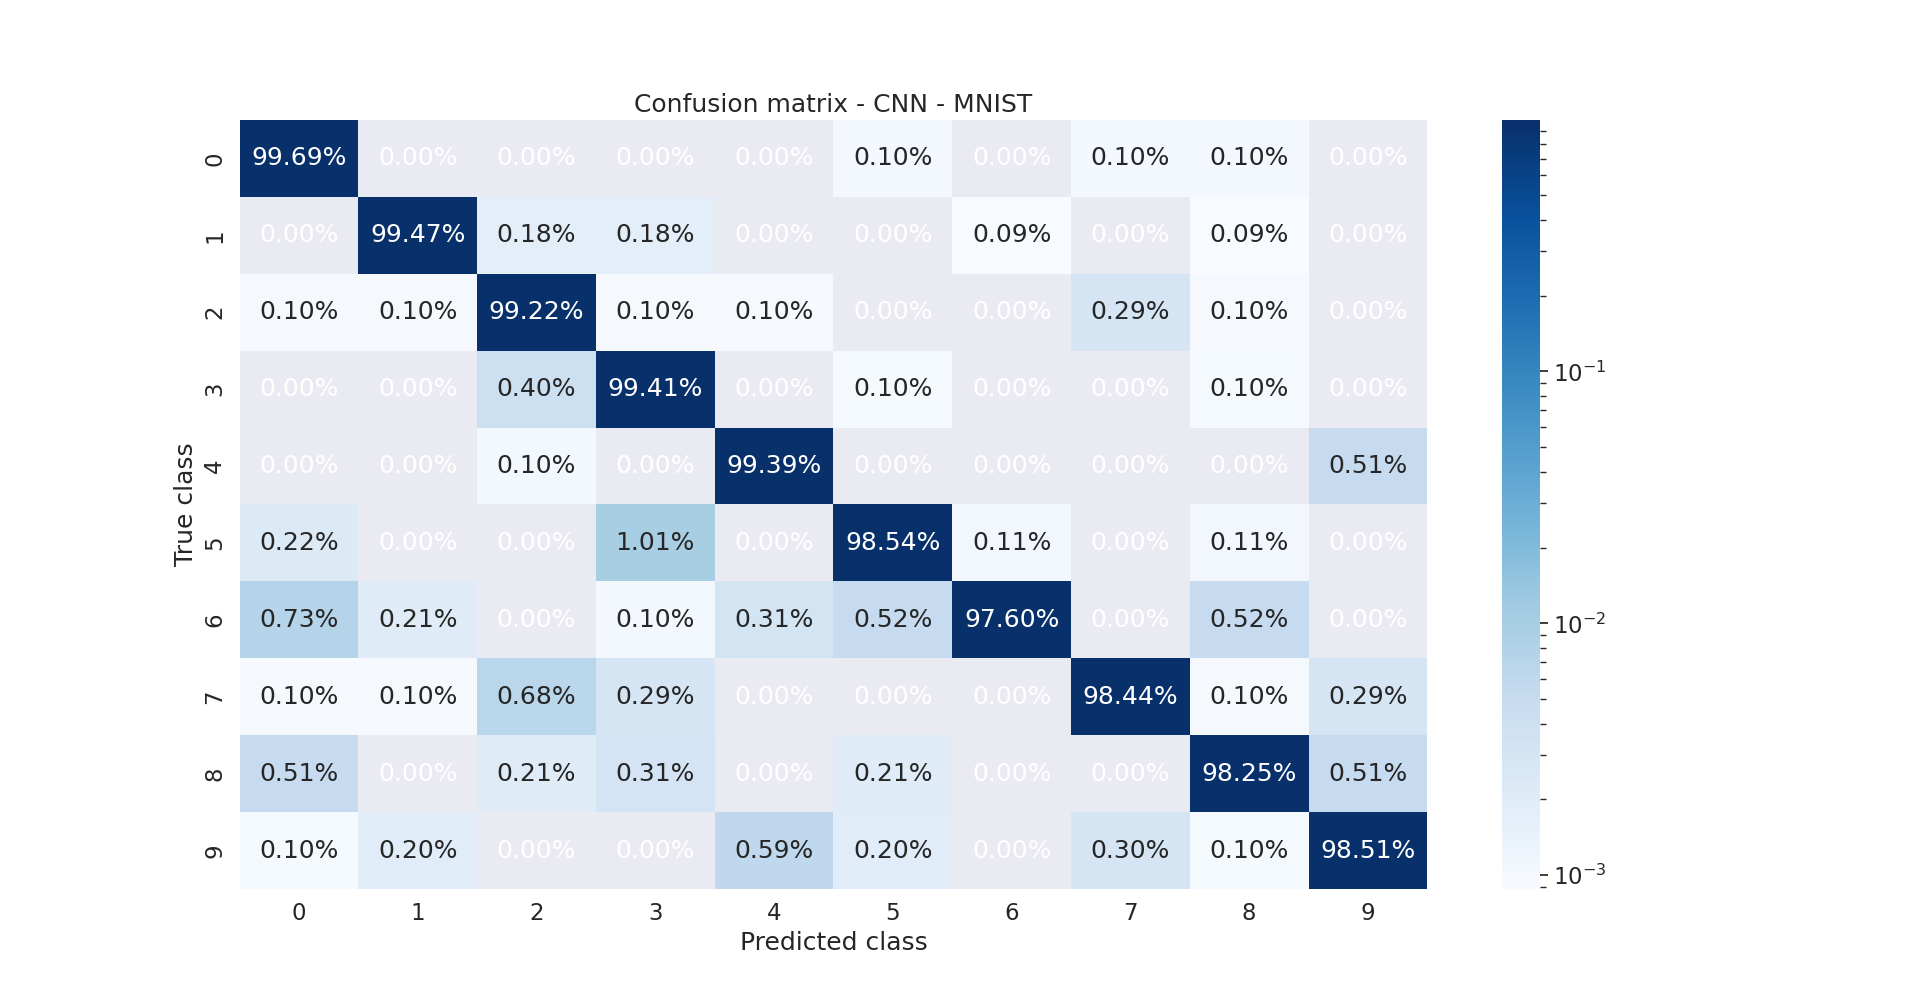
\includegraphics[width=8in]{figure/conf_cnn_MNIST.png}}
\caption{Confusion matrix for MNIST dataset classified using a CNN. From this figure, we can see that most misclassifications occur for digits that look similar: eights are sometimes misidentified as zeroes, and fours and nines are sometimes misidentified as eachother.}
\label{mnistheatmap_cnn}
\end{figure}

\subsubsection{Convolution followed by a Random Forest}

Given that we have achieved excellent results by using a CNN, we may don't expect to achieve much better results by sending the extracted features to a random forest. Regardless, our testing found that by using the same CNN model we found previously, 

\subsubsection{Principal Component Analysis followed by a Neural Network}

Replacing the convolutional stage with a simpler form of dimensionality reduction, namely PCA, we can see that we are able to reduce the dimensionality of our dataset while retaining a large amount of the information. Looking at figure~\ref{pcacomp}, we can see that even when using only the $50$ first principal components, the numbers are still readable. From this, we can assume that we can reduce the amount of features sent into our neural net from $784$ to less than $100$ features, and still expect reasonable results.

\begin{figure}[H]
\centerline{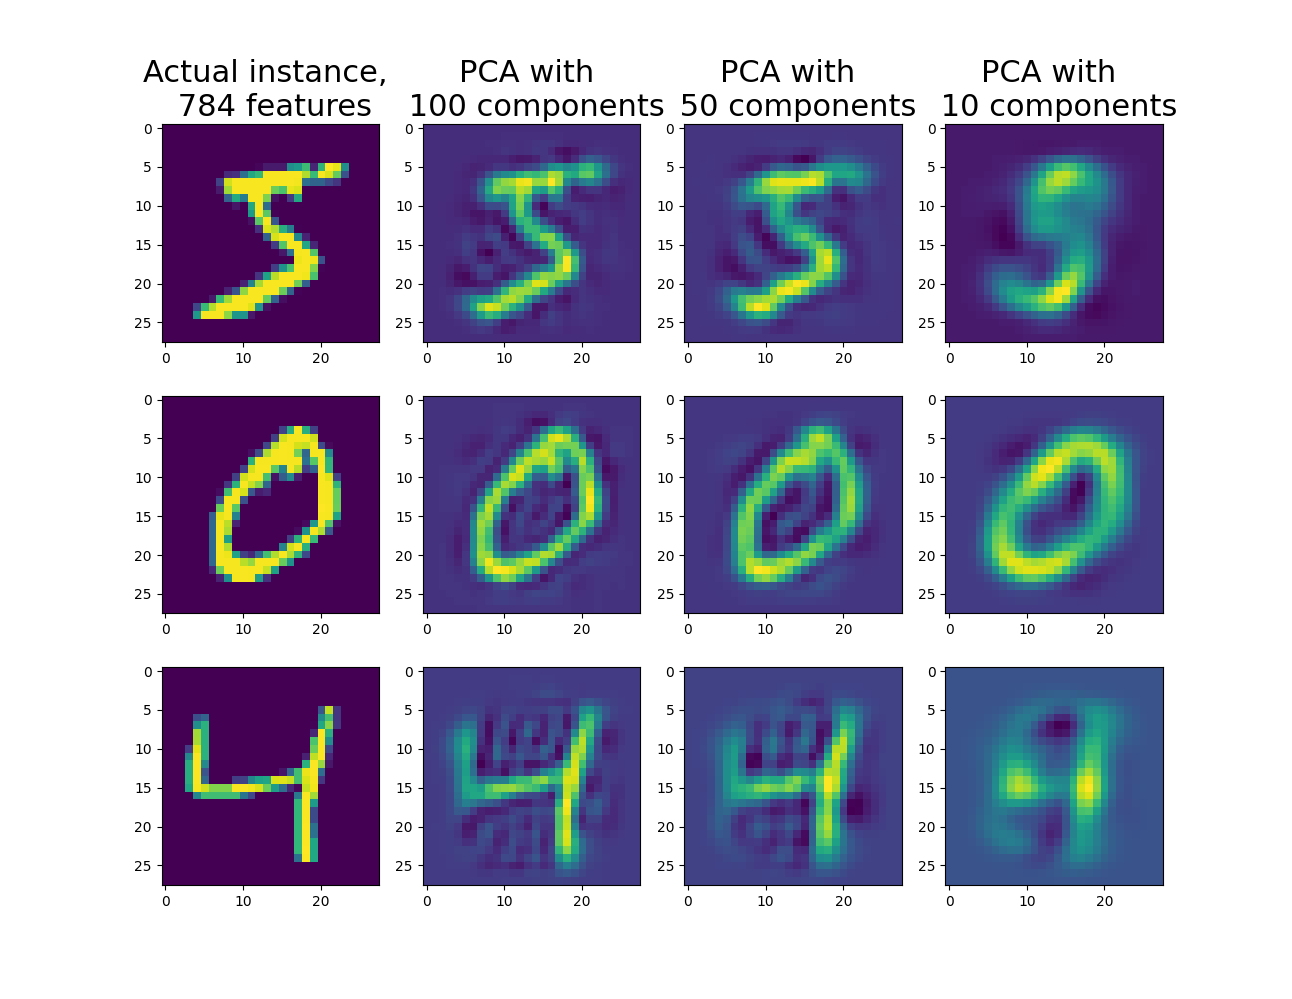
\includegraphics[width=5in]{figure/pcacomp.png}}
\caption{Comparison showing the amount of information lost by reducing the amount of principal components}
\label{pcacomp}
\end{figure}

Using different amount of principal components, we sent the reduced dataset into a neural network with three hidden layers. After testing different amounts of principal components to keep, and tuning the hyperparameters based on these, we found that even with only $50$ principal components, we achieved a test accuracy of $97.8\%$. This is comparable to the accuracy obtained by a traditional convolutional neural network. When considering the computational effort, we need to consider the performance benefit that modern GPU's bring, being specifically designed to run neural networks efficiently. This is very apparent in our testing: When using only a CPU, the PCA-NN model was much less intensive, requiring only $17$ seconds to complete training, while the convolutional neural network used $164$ seconds. This tells us that when computational resources are limited, simpler architectures can give reasonable results in a fraction of the time. However, when using a GPU with CUDA cores, the story is quite different: Here, the CNN used only $6$ seconds, while the PCA-NN model took $12$ seconds\footnote{The fact that this model took longer than the CNN is most likely because the PCA function we use only runs on the CPU, meaning that only the neural net part is actually running on the GPU}. Looking at the confusion matrix (Fig.~\ref{mnistheatmap_pcann}), we can see that we are again achieving very few misclassifications using the PCA-NN model.

\begin{figure}[H]
\centerline{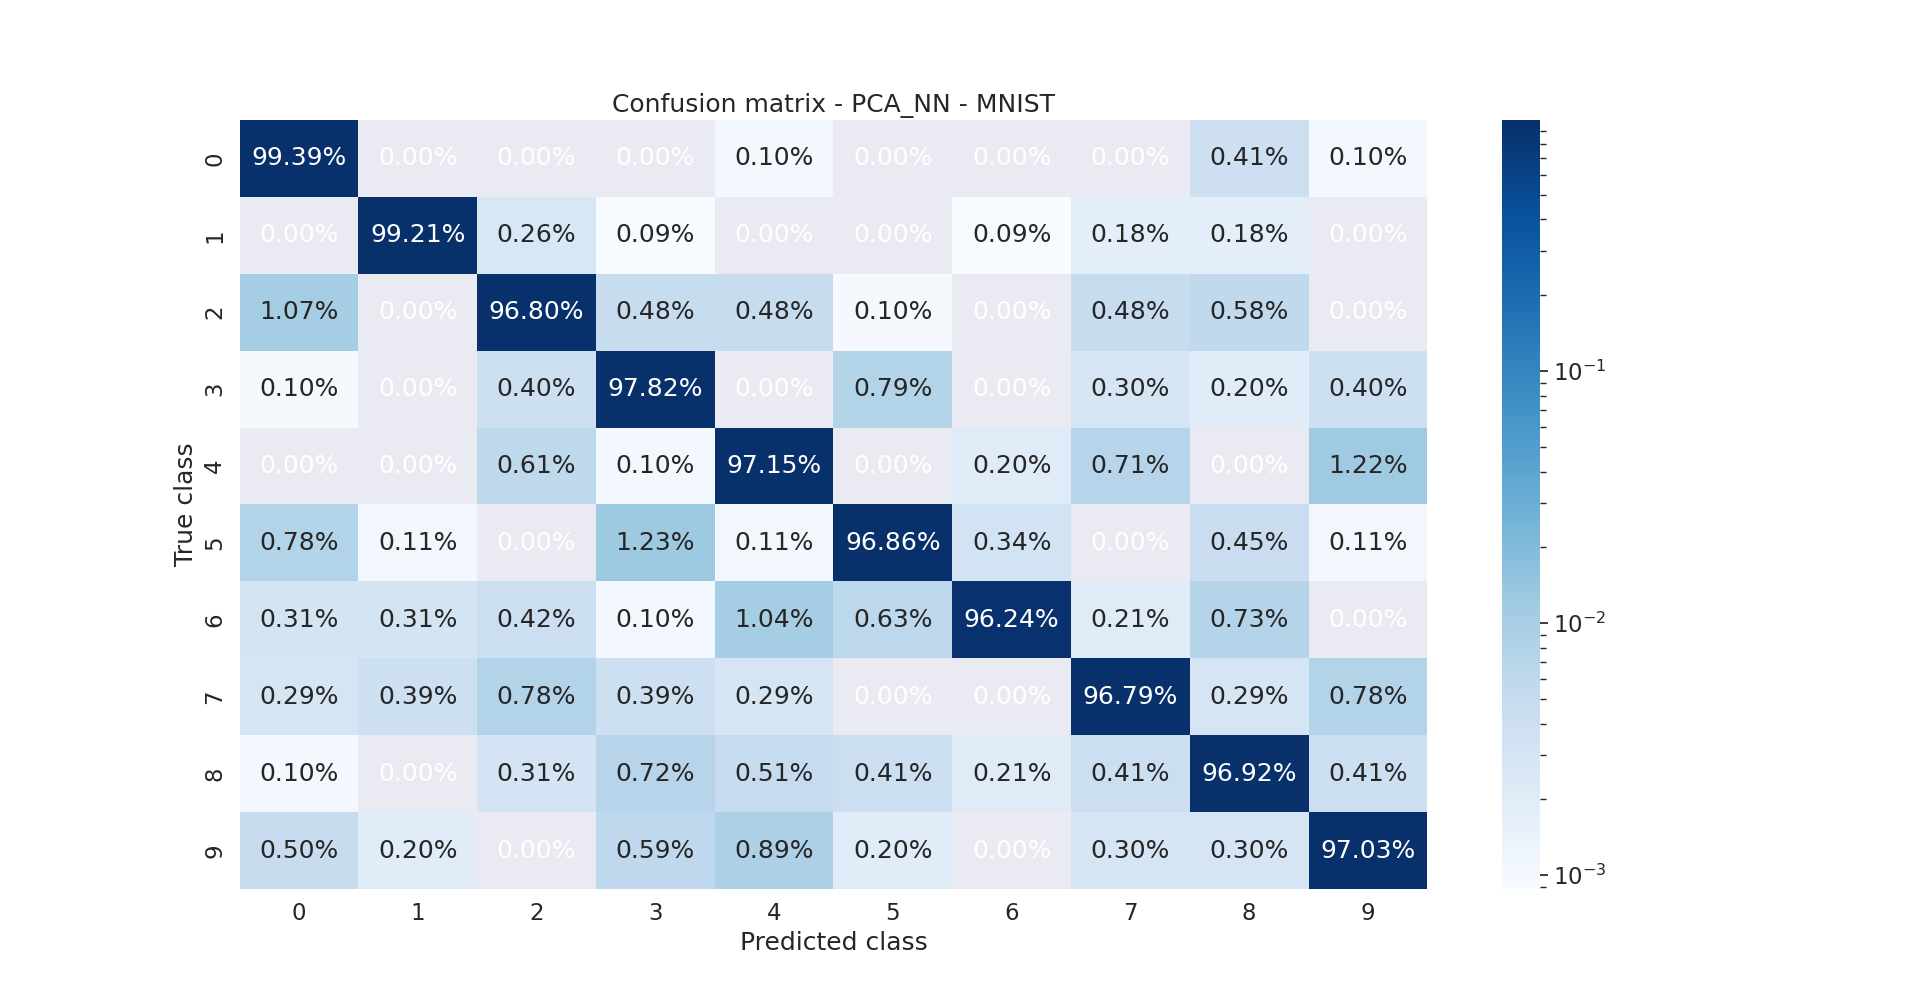
\includegraphics[width=8in]{figure/conf_pca_nn_MNIST.png}}
\caption{Confusion matrix for MNIST dataset classified using PCA followed by a neural network. Here we can see that misclassifications are slightly more common than when using a traditional CNN, but the results are still good.}
\label{mnistheatmap_pcann}
\end{figure}


\subsubsection{Principal Component Analysis followed by a Random Forest}

Satisfied with the results achieved by replacing the convolutional stage with Principal Component Analysis, we attempt to sidestep neural networks all together, and use PCA followed by a random forest. Here, we achieved a reasonable result of $94.7\%$ accuracy on the test set. Although this is not as impressive as the previous models, there

\subsection{Guangzhou Pneumonia Data}

As previously stated, the Guangzhou Pneumonia Dataset was collected and labeled as part of the article {\it Identifying Medical Diagnoses and Treatable Diseases by Image-Based Deep Learning}. In this article, the authors used transfer learning using a network previously trained on ImageNet to classify the x-ray images. With this method, they achieved a test accuracy of $92.8\%$ \cite[1127]{xray}. We now turn our attention to this dataset, and see if we can achieve similar results using our methods.

\subsubsection{Traditional Convolutional Neural Network}

Determining whether an x-ray shows a case of pneumonia or not is clearly a much more difficult classification problem than our previous dataset. Therefore, we initially had problems designing an architecture which achieved much higher than $80\%$ test accuracy. Clearly, we are not able to use a simple one convolutional layer model like we were able to on the MNIST dataset, and designing a general convolutional neural network architecture is a very complex task. Thus, we turn to the literature, and explore models which have been proven to be effective at image recognition. Out of the architectures presented in BOOK \cite{geron}, we decided to try AlexNet, which won the ILSVRC 2012 challenge and is a relatively shallow network having $11$ hidden layers. Using this model, we achieved a testing accuracy of $87.8\%$. Comparing our result to those obtained by Kermany et Al., we see that our model is slightly more ass.

\subsubsection{Convolution followed by a Random Forest}

\subsubsection{Principal Component Analysis followed by a Neural Network}

\subsubsection{Principal Component Analysis followed by a Random Forest}

\section{Conclusion}

% \begin{table}[h]
% \caption{Accuracy by }
% \begin{center}
% \label{datasettable}
% \begin{tabular}{| c | l | l | l |}
% \hline
% Dataset & Number of instances & Features & Type \\
% \hline
% Franke Function (raw data) & 400 & 2 & regression \\
% Franke Function (polynomial features) & 400 & 56 & regression \\
% Wisconsin Breast Cancer & 569 & 30 & binary classification \\
% MNIST 8x8 & 1797 & 64 & multiclass classification (10 classes) \\
% \hline
% \end{tabular}
% \end{center}
% \end{table}

I have realized that I am cooler than Eric.

The children of Guangzhou province were saved to a certain extent. They all lived happily ever after.

\bibliographystyle{apalike}
\bibliography{bibliography}

\section*{Appendix}

Here are some pictures of Eric Reber, formerly known as the criminal Ed "Gurgler" Bickley of Texas State Penistentiary.


\begin{figure}[h]
\centerline{\includegraphics[width=3.25in]{/home/jona/pictures/cat.jpg}}
\caption{Eric Reber in his most devious form}
\label{real1msetraintest}
\end{figure}


\end{document}
